% $Id$

%==============================================================================
\section{A Remote Component's Structure}
%==============================================================================

While we have implemented a local version of the Light Weight CORBA Component 
model $M_{CCM}$, the LwCCM specification defines remote components only.
Remote components are built up from CORBA objects that implement defined
IDL interfaces.
Because of the specified mapping from IDL3 to IDL2, the generated IDL2 files 
can be processed by every existing IDL compiler. In addition to CORBA stubs
and skeletons, remote component logic as well as CORBA component containers
must be implemented too. 

To be compliant to the LwCCM specification, we have developed a way to
adapt local components into remote LwCCM components - the 
{\it Local Component Adapter Concept} (LCAC).
LCAC allows to add remote communication
for each port transparently for business logic.
Fig.~\ref{LcacOverview} shows how a given local component implementation
can be extended to a remote LwCCM component.

\begin{figure}[htbp]
    \begin{center}
    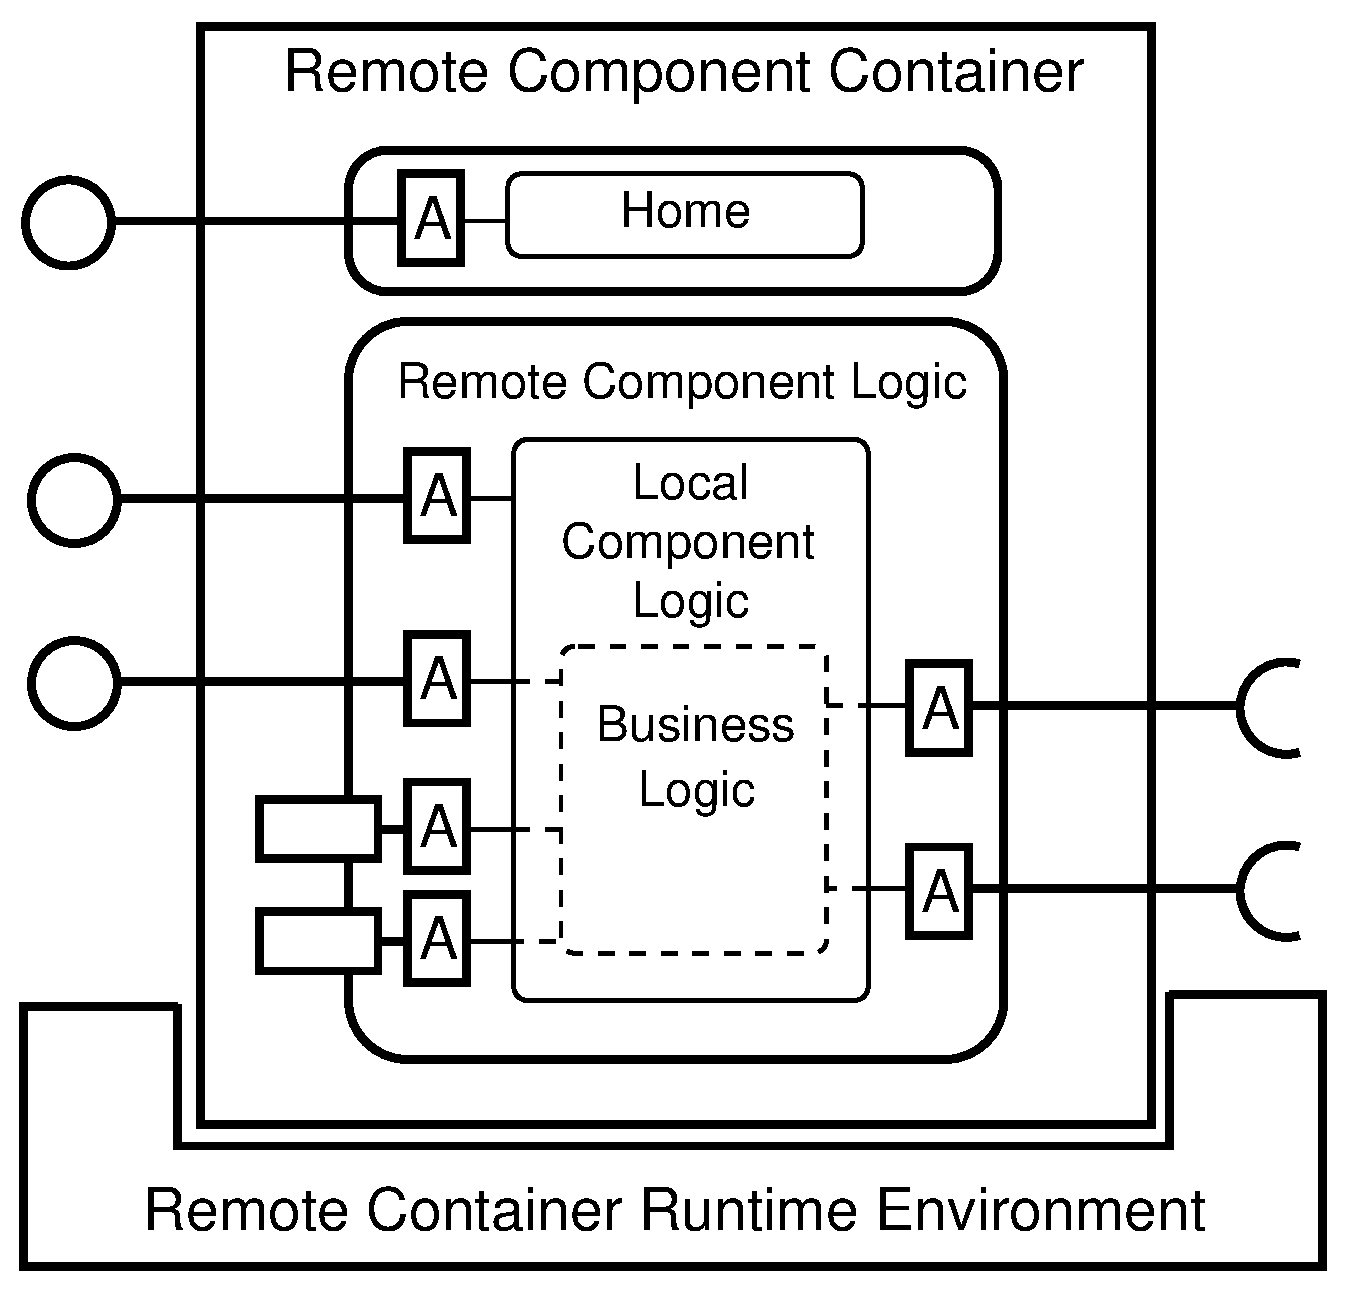
\includegraphics [width=5.5cm,angle=0] {figures/LocalAdapterConcept.eps}
    \caption{A local component can be embedded in a remote component logic
    that will be managed by a remote component container.}
    \label{LcacOverview}            
    \end{center}
\end{figure}

\noindent
The point is that we can use local components without changing them.
Thus, for a remote accessible component that provides at least one remote 
port, some additional code will be involved.

\begin{description}
\item [Remote component logic.]
A glue code layer is responsible for embedding a local component into a 
remote CORBA component. 
This remote component logic hosts the whole local component.
That means, its local component logic and business logic.  
Such a structure ensures that local ports can be used side by side to remote
ports.

\item [Adapter set.]
For a given IDL interface that defines a component port's syntax, a local and 
a remote implementation is generated. 
Using a set of adapter classes, these two worlds can fit together transparently.
In addition to component ports, adapters must be provided for component homes
as well as the component's equivalent interface.

\item [Remote component container.]
For each remote component type, a generic component container is used to
manage CORBA component instances.
In contrast to a local component container that can have a simple structure, a
remote container is also responsible for sophisticated {\it Quality of Service} 
(QoS) tasks.

\item [Remote container runtime environment.]
With increasing QoS functionality, the requirements to a remote container
runtime environment are growing too.
Besides an {\it Object Request Broker} (ORB), that handles CORBA requests,
libraries for multi--threading and process management implementation must 
be available.  
\end{description}

\noindent
This adapter concept is a powerful tool especially in heterogeneous 
environments. Besides the choice between local and remote connections, 
a deployment process can also decide to use different middleware technologies.


The fact that a local component is wrapped by a remote component becomes 
obvious from Fig.~\ref{StructureOfRemoteComponents}. All classes of a local
component remain unchanged, while some new ``remote'' classes have been added.

\begin{figure}[htbp]
    \begin{center}
    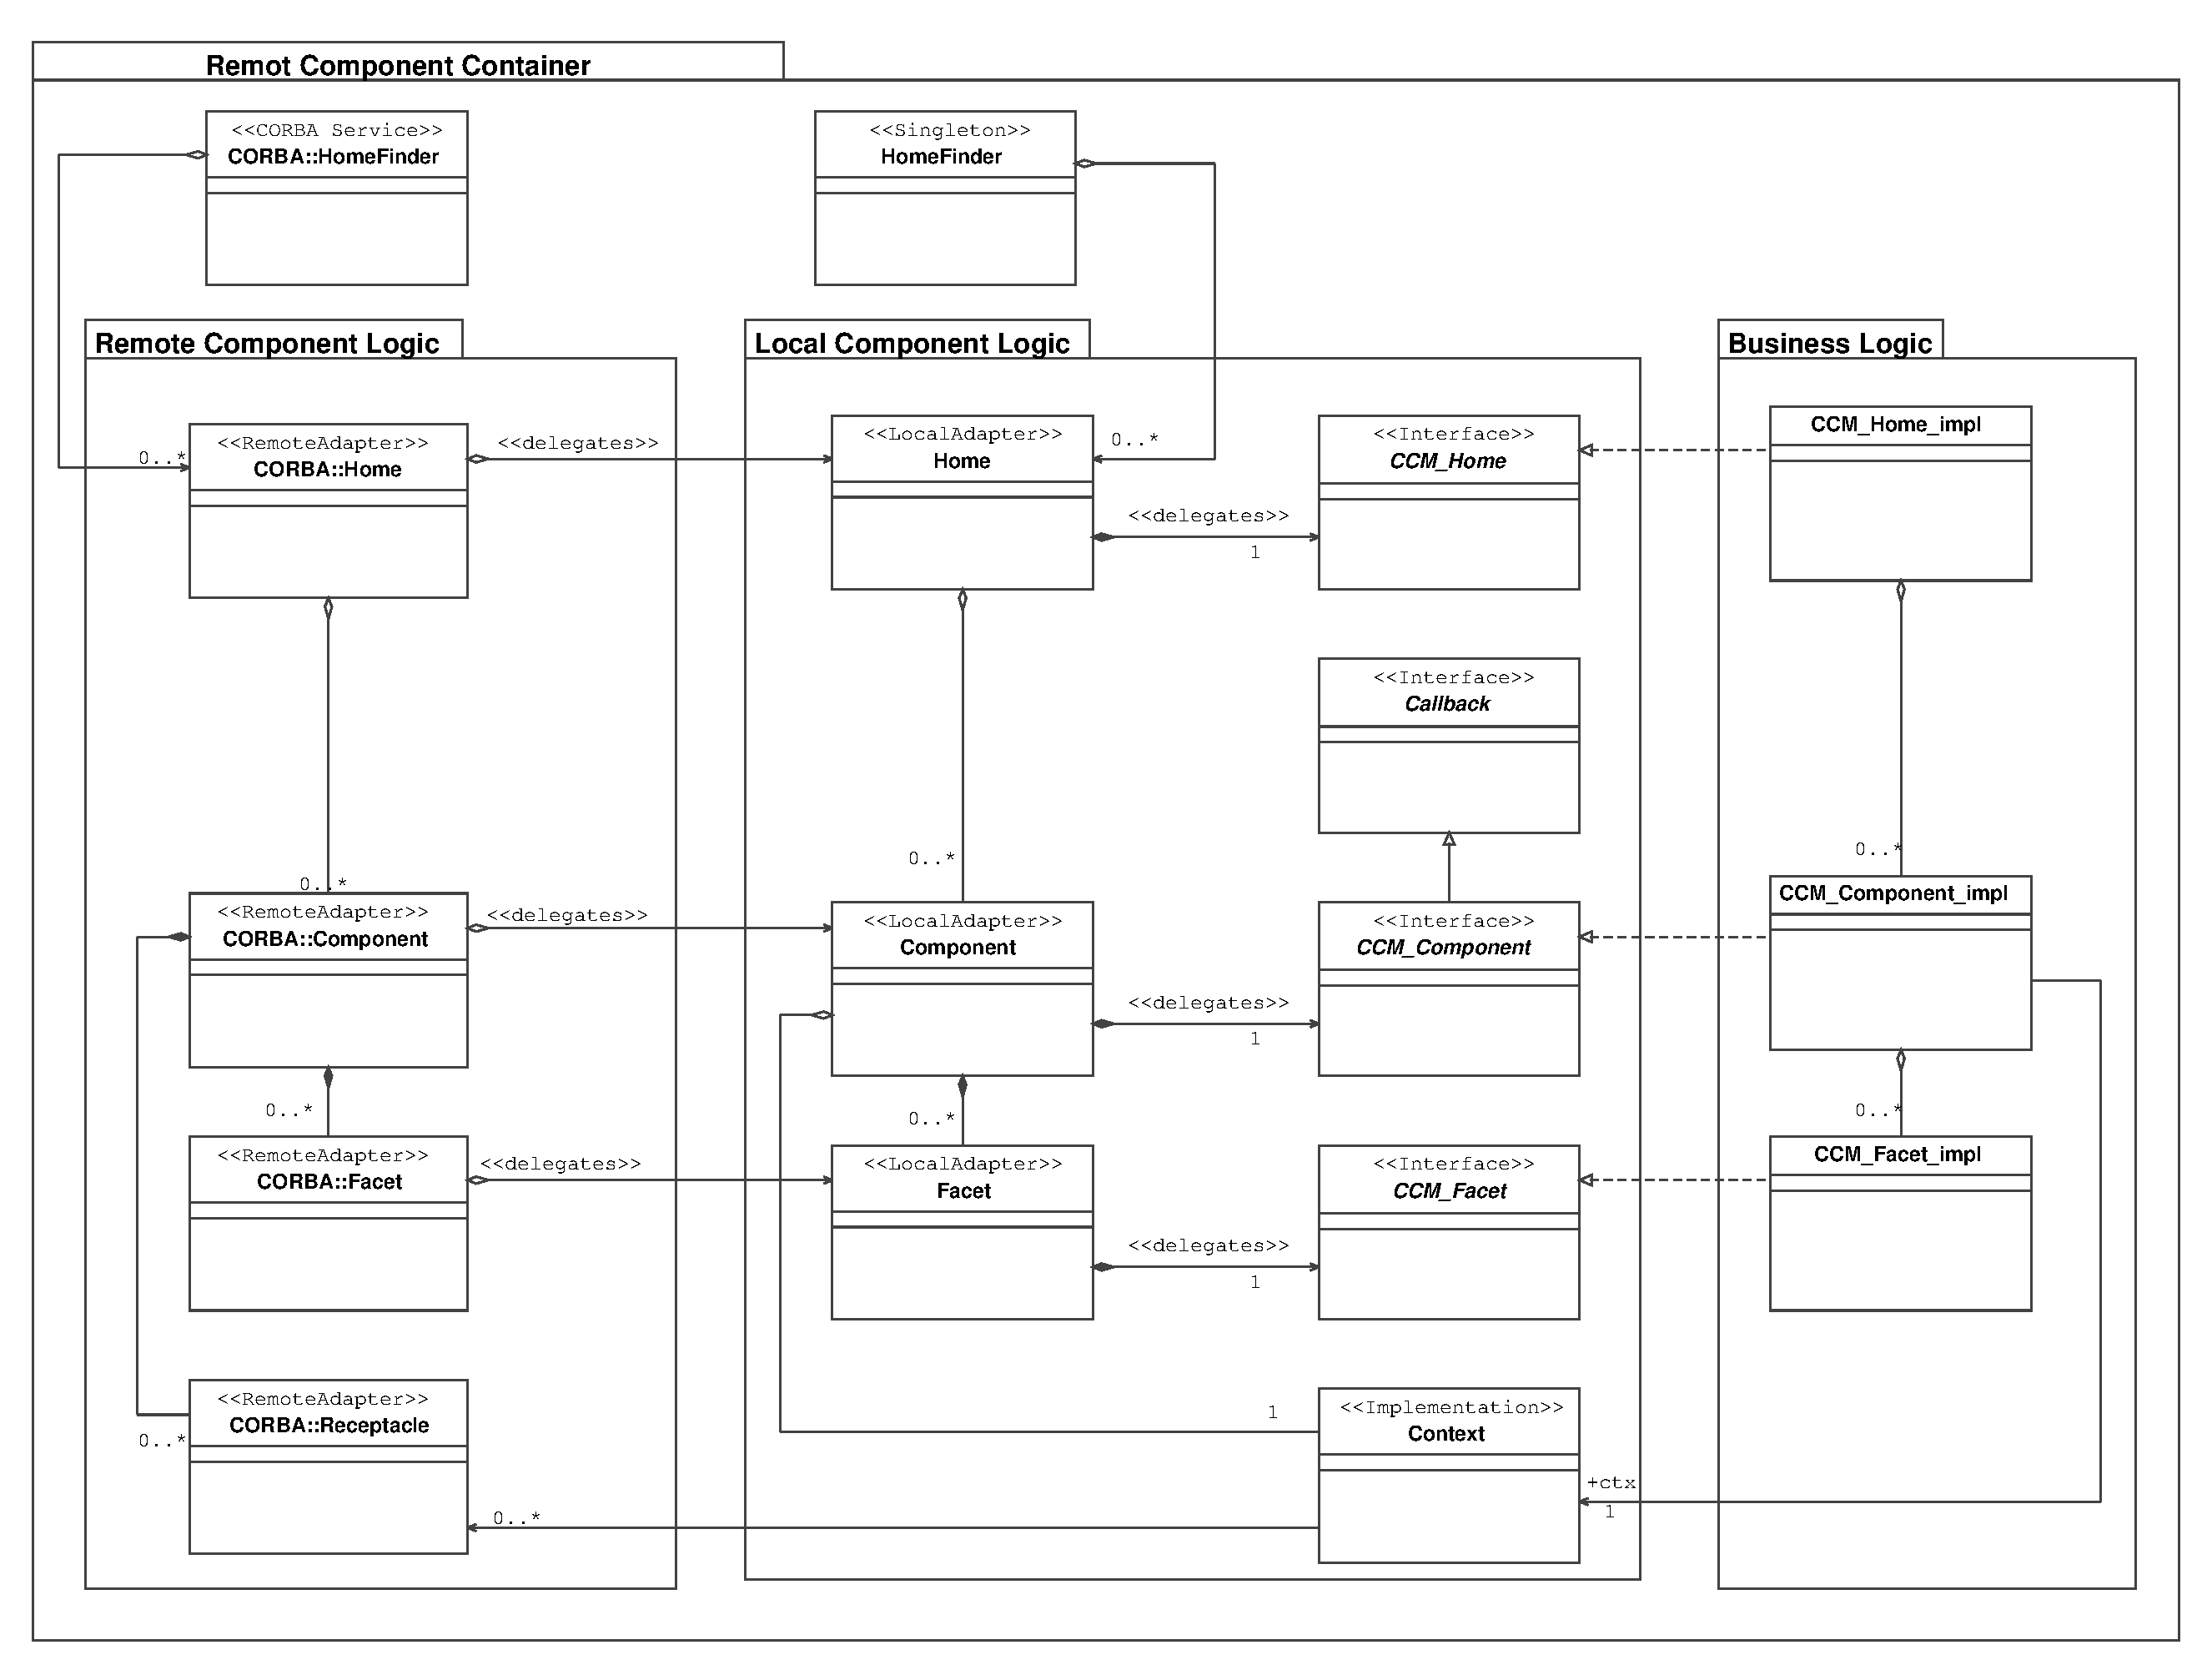
\includegraphics [width=15cm,angle=0] 
		     {uml/StructureOfRemoteComponents.eps}
    \caption{Simplified structure of a remote component implementation,
    showing the relationship between corresponding local and remote components.}
    \label{StructureOfRemoteComponents}            
    \end{center}
\end{figure}

\noindent
The remote structure is very similar to a local component's structure 
(Fig.~\ref{StructureOfLocalComponents}), thus, we can compare interactions
between a local and a remote component with interactions between business logic
and local component logic:

\begin{description}
\item [Calling component methods.]
A remote client calls methods on a remote adapter that delegates this
calls to a local component which uses a local adapter to delegate these calls
to business logic.
In each adapter, pre- and a post-invoke processing can take place 
(Fig.~\ref{RemoteComponentCall}).
\begin{figure}[htbp]
    \begin{center}
    \includegraphics [width=9cm,angle=0] 
		     {figures/RemoteComponentCall.eps}
    \caption{A remote call of a component's method is delegated twice
    allowing pre- and post-invoke processing.}
    \label{RemoteComponentCall}            
    \end{center}
\end{figure}

These two indirection layers allow non--functional extensions to 
components without changes in business logic. 
This separation of concerns is a cornerstone in component
based development.

\item [Invoking callback methods.]
Callback methods implemented by business logic can be
triggered either from local or remote component logic and their corresponding
container implementations to control a component's life cycle.



\item [Using context methods.]
Component business logic uses the {\tt Context} object to access container
functionality as well as component receptacles.
In the case of remote components, receptacles can be either local or remote
ports. Both kinds of receptacles can be accessed via local context
object methods. While local receptacles are connected directly to local facets,
remote receptacles are intercepted by a receptacle adapter.

\end{description}

\noindent
As a matter of course, a remote component implementation can also implement
nested component composition, contract verification and mirror component
tests.
Contrariwise, an existing LwCCM container implementation can be used to host 
local components, thus, we can combine an existing CORBA application server with
the presented extensions in the context of local components. 


\newpage
%------------------------------------------------------------------------------
\subsection{The designer's job}
%------------------------------------------------------------------------------

Of course, developing remote CORBA components starts with an IDL file. 
In fact, the
IDL comes from the CORBA stuff, and has already been used for local component 
development. 
To generate a remote layer around a local component, we can use existing IDL
files.
  
\begin{Example}
\begin{minifbox}
\begin{small}
\begin{verbatim}
interface Console {
  long println(in string s);
};

component Hello {
  attribute string prompt;
  provides Console console;
};

home HelloHome manages Hello {
};
\end{verbatim}
\end{small}
\end{minifbox}
\caption{Reusing the local component's IDL definition}
\label{example:one-component-idl}
\end{Example}


%------------------------------------------------------------------------------
\subsection{The developer's job}
%------------------------------------------------------------------------------

The basic idea is that a component developer always implements a local component.
Business logic is implemented in respect to the local component's programming
model without any CORBA in mind (and code ;-).
Thus, we start with implementing a local component as shown before:
\begin{small}
\begin{verbatim}
~/hello> ccmtools-c++-generate -d -c 2.0 -p hello2.0 Hello.idl
~/hello> ccmtools-c++-configure -p hello2.0
~/hello> ccmtools-c++-make -p hello1.0
\end{verbatim}
\end{small}

We implement the component's test, write the business logic, run the test and so on.
Remember, this iterative programming style forces short turn around cycles that are
not possible in a pure CORBA component environment.



%------------------------------------------------------------------------------
\subsubsection{Create the remote layer}
%------------------------------------------------------------------------------

To add a remote layer to an existing local component, we have to generate the
CORBA stubs and remote component adapters that join the CORBA objects with the
local component implementation.
All this code is generated using the following script:

\begin{small}
\begin{verbatim}
~/hello> ccmtools-c++remote-generate -d -p hello1.0 Hello.idl
\end{verbatim}
\end{small}
The {\tt ccmtools-c++remote-generate} script accepts the following command line
parameters:
\begin{itemize}
\item {\tt -d, -\-debug }\\
Enable debugging in generated code. The generated code produces a lot of debug
messages that can be used to trace the program execution. This also causes a
test client to be generated.

\item {\tt -p NAME, -\-package=NAME}\\
Set package name to NAME. The default package name is ``ccmtools-package''. Note
that the package name is used for the name of the generated subdirectory, unless
you override this behavior with the {\tt -o} option.

\item {\tt -h, -\-help}\\
Print out a short description of the available command line parameters.
\end{itemize}


\noindent
Beside the already existing directories and files of the local component code, 
now there are some new directories that contains the code for CORBA stubs and 
the remote component adapters.
Additionally, a second test file ({\tt \_check\_CCM\_Session\_*\_remote.cc}) is
created.

\begin{small}
\begin{verbatim}
    hello/
    |-- Hello.idl
    |-- _check_CCM_Session_Hello_remote.cc
    |-- hello1.0/
    |   |-- CCM_Session_Hello_remote
    |   |-- CCM_Test
    |   |-- idl2
\end{verbatim}
\end{small}

\noindent
We can build the local component code as well as the remote code with the
following commands:
\begin{small}
\begin{verbatim}
~/hello> ccmtools-c++-configure -p hello1.0
~/hello> ccmtools-c++-make -p hello1.0
\end{verbatim}
\end{small}
After the configure and build process, the local and the remote component tests
are started.
For the remote component test we use the CORBA collocation mechanism. Thus the 
generator  can implement the server and client code in a single test file.
Remember that to run the remote test a CORBA NameService must be established.


%------------------------------------------------------------------------------
\subsubsection{Deploy the remote component}
%------------------------------------------------------------------------------

To install the generated remote component library and header files in the
component repository, we can use the known CCM--Tools script:
\begin{verbatim}
~/hello> ccmtools-c++-install -p hello1.0
\end{verbatim}

\noindent
Applications can use the repository to access local or remote components 
like ordinary libraries.


%------------------------------------------------------------------------------
\subsubsection{Write a remote client and server}
%------------------------------------------------------------------------------

A remote component must be activated within a CORBA server application that
includes the header files of the ORB, the CORBA stubs and the remote
component.
\begin{Example}
\begin{minifbox}
\begin{small}
\begin{verbatim}
#include <CORBA.h>
#include <coss/CosNaming.h>

#include <CCM_Utils/Debug.h>
#include <CCM_Remote/CCM_Session_Hello/HelloHome_remote.h>
#include <Hello.h>

using namespace std;
using namespace CCM_Utils;
\end{verbatim}
\end{small}
\end{minifbox}
\caption{CORBA and remote component header files.}
\label{ServerHeaderFiles}
\end{Example}

\noindent
The remote {\tt Hello} component can be activated using the generated {\tt deploy\_HelloHome()} 
function. The first parameter is the initialized ORB object and the second parameter
defines the name of the component's home. This name is used to register the component's
home in the CORBA NameService. 
\begin{Example}
\begin{minifbox}
\begin{small}
\begin{verbatim}
int main (int argc, char *argv[])
{
  // Set debugging mode
  Debug::set_global(true); 

  // Initialize ORB and value type factories
  CORBA::ORB_var orb = CORBA::ORB_init(argc, argv);
  CCM::register_all_factories (orb);

  int error = deploy_HelloHome(orb, "HelloHome:1.0");
  if(!error) {
    cout << "Component is running..." << endl;
  }
  else {
    cerr << "ERROR: Can't start components!" << endl;
    assert(0);
  }

  // Wait for CORBA requests
  orb.run();
}
\end{verbatim}
\end{small}
\end{minifbox}
\caption{Remote component activation.}
\label{RemoteComponentServer}
\end{Example}

\noindent
Note that the ORB must be initialized and started before a remote component
can be accessed from a CORBA client.

\noindent
The remote client also has to initialize the ORB and the CORBA NameService,
as shown in Example \ref{ClientInit}.
\begin{Example}
\begin{minifbox}
\begin{small}
\begin{verbatim}
int main (int argc, char *argv[])
{
  Debug::set_global(true); 

  // Initialize ORB 
  CORBA::ORB_var orb = CORBA::ORB_init(argc, argv);
  CORBA::Object_var obj = 
    orb->resolve_initial_references ("NameService");
  CosNaming::NamingContextExt_var nc = 
    CosNaming::NamingContextExt::_narrow (obj);
\end{verbatim}
\end{small}
\end{minifbox}
\caption{Initialize the client's ORB and NameService.}
\label{ClientInit}
\end{Example}

From the CORBA NameService, the client gets a reference to the 
remote component's home. 
After narrowing the CORBA reference to the particular home type, 
the {\tt create()} method is used to get a component instance.
From the component instance we get a {\tt Console} facet reference, 
and set the {\tt prompt} attribute. 
A {\tt configuration\_complete()} call finishes the component 
configuration.

\begin{Example}
\begin{minifbox}
\begin{small}
\begin{verbatim}
  // Find ComponentHomes in the Naming-Service
  obj = nc->resolve_str ("HelloHome:1.0");
  HelloHome_var myHelloHome = HelloHome::_narrow (obj);

  // Create component instances
  Hello_var myHello =  myHelloHome->create();

  // Provide facets   
  Console_var console = myHello->provide_console();
	
  // Configure the component's attribute
  myHello->prompt("=->");

  // Component configuration finished	
  myHello->configuration_complete();
\end{verbatim}
\end{small}
\end{minifbox}
\caption{Creating the remote component and facet.}
\label{CreatingRemoteComponent}
\end{Example}

\noindent 
Now the remote client can use the component instance to call methods on
the component's equivalent interface and the supported facet.
%Every client request is forwarded to a CORBA object on the server side
%that workes as an adapter to the local component implementation. 
\begin{Example}
\begin{minifbox}
\begin{small}
\begin{verbatim}
  // Call operations on the component and its facets
  cout << "Version = " << 
    myHello->getComponentVersion() << endl;
  cout << "Date = " << 
    myHello->getComponentDate() << endl;

  console->println("Hello from the remote client");
\end{verbatim}
\end{small}
\end{minifbox}
\caption{Calling the remote component methods.}
\label{RemoteMethodCalling}
\end{Example}

\noindent
Finally, the remote client removes the component instance on the server side
and exits from the main function.

\begin{Example}
\begin{minifbox}
\begin{small}
\begin{verbatim}
  // Destroy component instances
  myHello->remove();
}
\end{verbatim}
\end{small}
\end{minifbox}
\caption{Destroy component instance.}
\label{DestroyComponent}
\end{Example}



%------------------------------------------------------------------------------
\subsubsection{Undeploy the remote component}
%------------------------------------------------------------------------------

To remove the component's libraries and header files from the repository, 
call:
\begin{verbatim}
~/hello> ccmtools-c++-uninstall -p hello1.0
\end{verbatim}
Remember, only the installed libraries and header files are deleted while
the developers source code remains untouched.


